% Replacing 5 by three strictly smaller values descends in the multiset order.
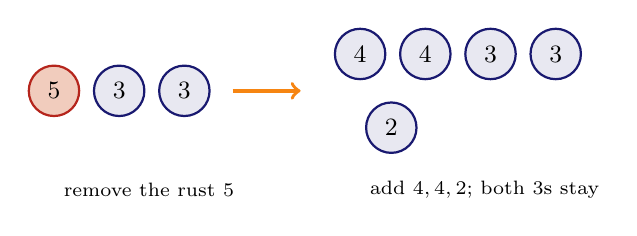
\begin{tikzpicture}[x=0.72cm,y=0.72cm,
  chip/.style={circle,draw=MidnightBlue,thick,fill=MidnightBlue!10,inner sep=0pt,minimum size=6.4mm,font=\small}]
  \node[chip,fill=BrickRed!18,draw=BrickRed] (a) at (0,0.9) {$5$};
  \node[chip] (b) at (1.15,0.9) {$3$};
  \node[chip] (c) at (2.3,0.9) {$3$};
  \draw[BurntOrange,line width=1.3pt,->] (3.15,0.9) -- (4.35,0.9);
  \node[chip] (d) at (5.4,1.55) {$4$};
  \node[chip] (e) at (6.55,1.55) {$4$};
  \node[chip] (g) at (7.7,1.55) {$3$};
  \node[chip] (h) at (8.85,1.55) {$3$};
  \node[chip] (f) at (5.95,0.25) {$2$};
  \node[font=\scriptsize,anchor=west] at (0,-0.85) {remove the rust $5$};
  \node[font=\scriptsize,anchor=west] at (5.4,-0.85) {add $4,4,2$; both $3$s stay};
\end{tikzpicture}
